\documentclass{article}
%  ╔══════════════════════════════════════════════════════════╗
%  ║                         Title                            ║
%  ╚══════════════════════════════════════════════════════════╝
%NOTE: I want \title,\author to be near top, and this \renewcommand{\maketitle} fails if these are above it.
\usepackage[utf8]{inputenc}         % Used to compile any UTF-8 Character (and supports Unicode)
\usepackage{titling}

\renewcommand{\maketitle}{
    \quad
    \vspace{1em}
  \begin{center}
      \LARGE\bfseries \thetitle \par
      \vspace{0.6em}
      \large
  \end{center}
    \vspace{1em}
}

\title{Clock Arithmetic and some Mysteries of Prime Numbers}
\author{Nathanael Chwojko-Srawley}
\date{\today}

%  ╔══════════════════════════════════════════════════════════╗
%  ║                         packages                         ║
%  ╚══════════════════════════════════════════════════════════╝

\usepackage{extarrows}         % Used to compile any UTF-8 Character (and supports Unicode)
\usepackage{stackengine}
\usepackage{colortbl}
\usepackage{scalerel}
\usepackage{amsmath, amssymb} % Used to write better mathematical expressions (ex. \mathbb{R})
\usepackage{stackrel}         % for left-right arrows, staking symbol above and bellow
\usepackage{mathrsfs}
\usepackage{euscript}
\usepackage[font=itshape]{quoting}
\usepackage{mathtools}
  \usepackage{enumitem}
\usepackage{amsthm}           % Used to create theorem enviroments.
\usepackage{graphicx}         % Let's you use images in LaTeX; ex the \includegraphics command.
\usepackage{hhline}
%\usepackage{luatexja}
%\usepackage{fontspec}
\usepackage{dsfont}
\usepackage{wasysym}          % emoji's!
\usepackage{float}            % package with ``H'' for figures and tables, ex. Images, tables, etc
%\usepackage{subcaption}      % More options with sub-captions.
\usepackage{setspace}         % More flexibility on spacing in document.
\usepackage{hyperref}         % let's me put hyperlinks
%\usepackage{tikz}             % for commutative diagrams https://tex.stackexchange.com/questions/419221/how-to-do-the-pushout-with-universal-property
\usepackage{tikz-cd}          % for commutative diagrams https://tex.stackexchange.com/questions/419221/how-to-do-the-pushout-with-universal-property
%\usepackage{quiver}           % for better commutative diagrams
\usepackage{bookmark}         % creating heading shortcut bar on the left as in word
\usepackage{longtable}        % create tables that extend past one page
%\usepackage{siunitx}         % required for alignment
%\usepackage{multirow}        % for multiple rows
\usepackage{microtype}        % makes nice text. Fixes some under-/over- filled box problems.
%\usepackage{fancyvrb}        % Let's you write code (different style than listings).
\usepackage[most]{tcolorbox} 	      % Makes nice boxes for thms, cor, prop, or anything else.
%\usepackage{enumitem}        % More flexibility on enumeration (don't know much).
\usepackage{xcolor}           % Colour text.
\usepackage{wrapfig}          % To wrap text around figure
\usepackage{listings}         % Create nice colour code blocks (customized in preamble)
\usepackage{thmtools}         % Customize theorem environment (in preamble).
%\usepackage{marvosym}        % Provide ``basic'' symbols (hazard, religious, smiley face etc.)
\usepackage{array}            % \begin{table}{>{\em}c c} -> 1st column italic (bfseries for bold)
%\usepackage[english]{babel}  % If I want to blindtext in english.
\usepackage{blindtext}
\usepackage[a4paper, total={6in, 8.5in}]{geometry}
%\usepackage[symbol]{footmisc} % For daggers and asterisk for footnotes. 1: *, 2: dagger, etc.
\usepackage{fancyhdr}
\usepackage{titlesec}
%\usepackage{pst-plot}          %To make nice plots: https://tex.stackexchange.com/questions/47594/how-can-i-make-a-graph-of-a-function#47596
% \usepackage[answerdelayed]{exercise}
\usepackage{etoolbox}          % for Dynkin diagrams
\usepackage{dynkin-diagrams}   % for Dynkin diagrams

% \usepackage{CJKutf8} % for some chinese


% \renewcommand{\thesection}{\arabic{section}}
%header information
\pagestyle{fancy}

\setlength\headheight{20pt}

\renewcommand{\sectionmark}[1]{\markright{\thesection.\ #1}}

\fancyfoot[C,CO]{\textcolor{gray}{Nathanael Chwojko-Srawley}}
\fancyfoot[R,RO]{\thepage}{}

% Create a new page style for the first page
\fancypagestyle{firstpage}{
  \fancyhf{} % Clear header and footer
  \fancyhead[L]{\theauthor}
  \fancyhead[R]{\today} % Date in the top-right
  \fancyfoot[C]{\textcolor{gray}{Nathanael Chwojko-Srawley}}
  \fancyfoot[R]{\thepage}
}

% Apply the first page style conditionally
\AtBeginDocument{\thispagestyle{firstpage}}


\newcommand{\chapter}[1]{%
  \clearpage
  \vspace*{30pt} % Space before the chapter title
  {\normalfont\huge\bfseries #1\par} % Chapter title formatting
  \vspace{20pt} % Space after the chapter title
}


\newcommand\scalemath[2]{\scalebox{#1}{\mbox{\ensuremath{\displaystyle #2}}}}
\newcommand{\Equiv}[1]{\equiv_{\scalemath{0.6}{#1}}}
\newcommand{\Plus}[1]{+_{\scalemath{0.6}{#1}}\,}
\newcommand{\Minus}[1]{-_{\scalemath{0.6}{#1}}\,}
\newcommand{\Cdot}[1]{\cdot{\scalemath{0.6}{#1}}\,}
%  ╔══════════════════════════════════════════════════════════╗
%  ║                     Custom Commands                      ║
%  ╚══════════════════════════════════════════════════════════╝

% mathbb
\newcommand{\A}{\mathbb{A}}
\newcommand{\C}{\mathbb{C}}
\newcommand{\F}{\mathbb{F}}
\newcommand{\N}{\mathbb{N}}
\newcommand{\Q}{\mathbb{Q}}
\newcommand{\R}{\mathbb{R}}
\newcommand{\V}{\mathbb{V}}
\newcommand{\Z}{\mathbb{Z}}
\renewcommand{\H}{\mathbb{H}}

% mathcal
\newcommand{\co}{\mathfrak{o}} %mathcal{o} looks like wreath product, so I changed it to mathfrak
\newcommand{\CA}{\mathcal{A}}
\newcommand{\CB}{\mathcal{B}}
\newcommand{\CC}{\mathcal{C}}
\newcommand{\CD}{\mathcal{D}}
\newcommand{\CF}{\mathcal{F}}
\newcommand{\CG}{\mathcal{G}}
\newcommand{\CH}{\mathcal{H}}
\newcommand{\CI}{\mathcal{I}}
\newcommand{\CL}{\mathcal{L}}
\newcommand{\CN}{\mathcal{N}}
\newcommand{\CO}{\mathcal{O}}
\newcommand{\CP}{\mathbb{C}\mathrm{P}}
\newcommand{\CQ}{\mathcal{Q}}
\newcommand{\CR}{\mathcal{R}}
\newcommand{\CK}{\mathcal{K}}
\newcommand{\CS}{\mathcal{S}}
\newcommand{\CT}{\mathcal{T}}
\newcommand{\CV}{\mathcal{V}}
\newcommand{\CZ}{\mathcal{Z}}

%mathscr
\newcommand{\ff}{\mathscr{F}}

%Euscript
\newcommand{\EF}{\EuScript{F}}
\newcommand{\EL}{\EuScript{L}}
\newcommand{\EO}{\EuScript{O}}
\newcommand{\EC}{\EuScript{C}}

%mathfrak (lowercase)
\newcommand{\fa}{\mathfrak{a}}
\newcommand{\fb}{\mathfrak{b}}
\newcommand{\fc}{\mathfrak{c}}
\newcommand{\fd}{\mathfrak{d}}
\newcommand{\fm}{\mathfrak{m}}
\newcommand{\fn}{\mathfrak{n}}
\newcommand{\fo}{\mathfrak{o}}
\newcommand{\fp}{\mathfrak{p}}
\newcommand{\fq}{\mathfrak{q}}

%mathfrak (upper case)
\newcommand{\FA}{\mathfrak{A}}
\newcommand{\FB}{\mathfrak{B}}
\newcommand{\FP}{\mathfrak{P}}
\newcommand{\FC}{\mathfrak{C}}
\newcommand{\FD}{\mathfrak{D}}
\newcommand{\FM}{\mathfrak{M}}
\newcommand{\FN}{\mathfrak{N}}
\newcommand{\FO}{\mathfrak{O}}

% operatorname
\newcommand{\ev}{\operatorname{ev}}
\newcommand{\tr}{\operatorname{tr}}
\newcommand{\nm}{\operatorname{Nm}}
\newcommand{\op}{\operatorname{op}}
\newcommand{\ad}{\operatorname{ad}}
\newcommand{\im}{\operatorname{im}}
\newcommand{\id}{\operatorname{id}}
\newcommand{\ch}{\operatorname{ch}}
\newcommand{\ab}{\operatorname{ab}}
\newcommand{\SL}{\operatorname{SL}}
\newcommand{\GL}{\operatorname{GL}}
\renewcommand{\Re}{\operatorname{Re}}
\renewcommand{\Im}{\operatorname{Im}}
\newcommand{\rad}{\operatorname{rad}}
\newcommand{\vol}{\operatorname{vol}}
\newcommand{\Gal}{\operatorname{Gal}}
\newcommand{\Rep}{\operatorname{Rep}}
\newcommand{\Aut}{\operatorname{Aut}}
\newcommand{\Sym}{\operatorname{Sym}}
\newcommand{\Mod}{\operatorname{Mod}}
\newcommand{\Grp}{\operatorname{Grp}}
\newcommand{\Hom}{\operatorname{Hom}}
\newcommand{\Emb}{\operatorname{Emb}}
\newcommand{\Ext}{\operatorname{Ext}}
\newcommand{\End}{\operatorname{End}}
\newcommand{\Inn}{\operatorname{Inn}}
\newcommand{\Ind}{\operatorname{Ind}}
\newcommand{\Out}{\operatorname{Out}}
\newcommand{\Jac}{\operatorname{Jac}}
\newcommand{\Nil}{\operatorname{Nil}}
\newcommand{\Tor}{\operatorname{Tor}}
\newcommand{\Ann}{\operatorname{Ann}}
\newcommand{\Syl}{\operatorname{Syl}}
\newcommand{\Res}{\operatorname{Res}}
\newcommand{\lcm}{\operatorname{lcm}}
\newcommand{\conj}{\operatorname{conj}}
\newcommand{\disc}{\operatorname{disc}}
\newcommand{\stab}{\operatorname{stab}}
\newcommand{\kdim}{\operatorname{kdim}}
\newcommand{\coker}{\operatorname{coker}}
\newcommand{\Obj}{\operatorname{Obj}}
\newcommand{\Mor}[1]{\operatorname{Mor}(\textbf{#1})}
\newcommand{\Frac}{\operatorname{Frac}}
\newcommand{\Frob}{\operatorname{Frob}}
\newcommand{\Spec}{\operatorname{Spec}}
\newcommand{\mSpec}{\operatorname{mSpec}}
\newcommand{\Char}{\operatorname{char}}
\newcommand{\fHom}[1]{\operatorname{Hom}(#1, \_\_)}
\newcommand{\cofHom}[1]{\operatorname{Hom}(\_\_, #1)}
\newcommand{\trdeg}{\operatorname{trdeg}}
\newcommand{\Span}{\operatorname{span}}

%shorthands
\renewcommand{\bf}[1]{\textbf{#1}}
\newcommand{\qn}{\quad\newline}
\newcommand{\oln}{\overline}
\renewcommand{\phi}{\varphi}
\newcommand{\placeholder}{\_\_\_\_\_}
\newcommand{\set}[2]{\left\{#1 \ \middle|\ #2\right\}}

% connectors
\renewcommand{\mid}{\big|}
\newcommand{\sse}{\subseteq}
\newcommand{\subg}{\leqslant}
\newcommand{\supg}{\geqslant}
\newcommand{\ssne}{\subsetneq}
\newcommand{\isosubg}{\lesssim}
\newcommand{\nsse}{\not\subseteq}
\newcommand{\nsubg}{\trianglelefteq}
\newcommand{\nsupg}{\trianglerighteq}
\newcommand{\csubg}{\blacktriangleleft}
%\newcommand{\subgne}{\lneqslant}

% limits
\newcommand{\Lim}{\varprojlim}
\newcommand{\colim}{\varinjlim}
\newcommand{\coLim}{\varinjlim}
\newcommand{\Dlim}{\lim\limits_{\longrightarrow}}
\newcommand{\coDlim}{\lim\limits_{\longleftarrow}}


%for saturated ideals in the localization section (I don't like these, I think I'll delete)
\newcommand{\LIm}{{}^{\iota} }
\newcommand{\LPre}{{}^{\pi} }

% Arrows
\newcommand{\rw}{\rightarrow}
\newcommand{\Rw}{\Rightarrow}
\newcommand{\lw}{\leftarrow}
\newcommand{\Lw}{\Leftarrow}
\newcommand{\lrw}{\leftrightarrow}
\newcommand{\LRw}{\Leftrightarrow}
\newcommand{\rrw}{\rightrightarrows}
\newcommand{\acton}{\curvearrowright}
\newcommand{\actson}{\curvearrowright}
\newcommand\mapsfrom{\mathrel{\reflectbox{\ensuremath{\mapsto}}}}

% dcups
\newcommand{\dcup}{\sqcup}
\newcommand{\Dcup}{\bigsqcup}

%a nice large circle
\newcommand{\tikzcircle}[2][red,fill=black]{\tikz[baseline=-0.5ex]\draw[#1,radius=#2] (0,0) circle ;}%
\makeatletter
\newcommand*\bigcdot{\mathpalette\bigcdot@{2}}
\newcommand*\bigcdot@[2]{\mathbin{\vcenter{\hbox{\scalebox{#2}{$\m@th#1\bullet$}}}}}
\makeatother

%somehow not a default command
\def\rddots{\mathstrut^{.^{.^{.}}}}

%% new delimiter
\DeclarePairedDelimiter{\ceil}{\lceil}{\rceil}


%  ╔══════════════════════════════════════════════════════════╗
%  ║                          proofs                          ║
%  ╚══════════════════════════════════════════════════════════╝
\usepackage{tikz-cd}          % for commutative diagrams https://tex.stackexchange.com/questions/419221/how-to-do-the-pushout-with-universal-property
\def\exampletext{Exercise} % If English
\colorlet{colexam}{red!55!black} % Global example color


\newtcbtheorem{exercise}{Exercise}{% \newtcolorbox[use counter=testexample]{testexamplebox}{%
% Example Frame Start
empty,% Empty previously set parameters
title={\exampletext \thetcbcounter #1},% use \thetcbcounter to access the testexample counter text
% Attaching a box requires an overlay
attach boxed title to top left,
   % Ensures proper line breaking in longer titles
   minipage boxed title,
% (boxed title style requires an overlay)
boxed title style={empty,size=minimal,toprule=0pt,top=4pt,left=3mm,overlay={}},
coltitle=colexam,fonttitle=\bfseries,
before=\par\medskip\noindent,parbox=false,boxsep=0pt,left=3mm,right=0mm,top=2pt,breakable,pad at break=0mm,
   before upper=\csname @totalleftmargin\endcsname0pt, % Use instead of parbox=true. This ensures parskip is inherited by box.
% Handles box when it exists on one page only
overlay unbroken={\draw[colexam,line width=.5pt] ([xshift=-0pt]title.north west) -- ([xshift=-0pt]frame.south west); },
% Handles multipage box: first page
overlay first={\draw[colexam,line width=.5pt] ([xshift=-0pt]title.north west) -- ([xshift=-0pt]frame.south west); },
% Handles multipage box: middle page
overlay middle={\draw[colexam,line width=.5pt] ([xshift=-0pt]frame.north west) -- ([xshift=-0pt]frame.south west); },
% Handles multipage box: last page
overlay last={\draw[colexam,line width=.5pt] ([xshift=-0pt]frame.north west) -- ([xshift=-0pt]frame.south west); }%
}{ex}


\def\prooftext{Proof} % If English
\NewDocumentEnvironment{Proof}{ O{} }
{
  \colorlet{colexam}{black!55!black} % Global example color
  \newtcolorbox[number within=section]{testproofbox}{% \newtcolorbox[use counter=testexample]{testexamplebox}{%
    % Example Frame Start
    empty,% Empty previously set parameters
    title={\emph{\prooftext} \thetcbcounter: #1},% use \thetcbcounter to access the testexample counter text
    % Attaching a box requires an overlay
    attach boxed title to top left,
       % Ensures proper line breaking in longer titles
       minipage boxed title,
    % (boxed title style requires an overlay)
    boxed title style={empty,size=minimal,toprule=0pt,top=4pt,left=3mm,overlay={}},
    coltitle=colexam,fonttitle=\bfseries,
    before=\par\medskip\noindent,parbox=false,boxsep=0pt,left=3mm,right=0mm,top=2pt,breakable,pad at break=0mm,
       before upper=\csname @totalleftmargin\endcsname0pt, % Use instead of parbox=true. This ensures parskip is inherited by box.
    % Handles box when it exists on one page only
    overlay unbroken={\draw[colexam,line width=.5pt] ([xshift=-0pt]title.north west) -- ([xshift=-0pt]frame.south west); },
    % Handles multipage box: first page
    overlay first={\draw[colexam,line width=.5pt] ([xshift=-0pt]title.north west) -- ([xshift=-0pt]frame.south west); },
    % Handles multipage box: middle page
    overlay middle={\draw[colexam,line width=.5pt] ([xshift=-0pt]frame.north west) -- ([xshift=-0pt]frame.south west); },
    % Handles multipage box: last page
    overlay last={\draw[colexam,line width=.5pt] ([xshift=-0pt]frame.north west) -- ([xshift=-0pt]frame.south west); },%
    }
  \begin{testproofbox}
}
{\end{testproofbox}\endlist}

\newtcbtheorem[number within=section]{titledBox}{}{%
  enhanced,
  sharp corners,
  colback=white,
  colframe=black,
  borderline={0.2pt}{0pt}{black},
  left=2mm,
  right=2mm,
  top=2mm,
  bottom=2mm,
  title style={opacity=1},
  attach title to upper,
  before upper={\textbf{\tcbtitletext}\quad},
  coltitle=black,
  fonttitle=\bfseries,
  separator sign={\quad}
}{box}
\setlength{\parindent}{0pt} % don't like indentation infront of paragraphs
\setlength{\parskip}{1ex}   %so that there is still space between paragarphs

% \usepackage[backend=biber,citestyle=alphabetic,bibstyle=authortitle]{biblatex}
\usepackage{biblatex}

\addbibresource{bibliography.bib}

\makeatletter
\def\blfootnote{\gdef\@thefnmark{}\@footnotetext}
\makeatother


\definecolor{dkgreen}{rgb}{0,0.6,0}
\definecolor{gray}{rgb}{0.5,0.5,0.5}
\definecolor{mauve}{rgb}{0.58,0,0.82}
\definecolor{lightyellow}{rgb}{1,1,0.6}
\definecolor{reddish}{HTML}{A01A3A}

\definecolor{LinkColour}{HTML}{A64A3B} % favourite
% \definecolor{LinkColour}{HTML}{8C3D32} % 2nd place
\hypersetup{
  colorlinks,
  citecolor=black,
  filecolor=magenta,
  linkcolor=LinkColour,
  urlcolor=blue,
}

\setcounter{secnumdepth}{1}  % start numbering at section, no chapter

\begin{document}
\maketitle

\vspace{2em}
This article is written for my patient friends to whom I give math riddles that require knowledge of modular
arithmetic, or as I often call it \emph{clock arithmetic}. This article serves as an easy reference for the
necessary concepts and requires no mathematical background. For this entire article, we will only care about
which hour the hour-hand is on; no AM or PM, and no adding half an hour (or anything that isn't an increment
of 60 minutes).

\qn
All exercises and applications can be skipped; they are there for fun!
\vspace{2em}

\section{Clock Arithmetic: Addition and Multiplication}


We all have (at least) two ideas of addition in our heads. The first one is the usual notion of adding
quantities\footnote{A mathematician would say \emph{discrete quantities} to distinguish from
  \emph{continuous} quantities, which would describe something like water where the amount we add is on a
``continuous'' spectrum of possible amounts rather than ``discrete'' indivisible chunks of amounts}: If I have
$4$ bottles and add $10$ bottles, I have $14$ bottles. In other words
\[
  4+10 = 14
\]
The other notion of addition we often use is when we are calculating what time it is. Consider a
$12$-hour clock. If it is $4$ o'clock, in $5$ hours it will be $9$ o'clock. If instead we add $10$ hours, it
will be $2$ o'clock. In other words, we comfortably did
\[
  4+10 = 2
\]
in our heads. This is certainly different than the previous equality, but it still makes sense! Using the same symbol ``$+$''
may cause confusion, so to distinguish the two types of addition, we shall write $+_{12}$ for ``12 hour
clock'' addition, and keep $+$ for quantity addition. Thus, we can write:
\[
  4+10 = 14 \qquad \text{and} \qquad 4+_{12}10 = 2
\]
Let us call the addition using $+$ \emph{natural arithmetic} and the addition using $+_{12}$
\emph{clock arithmetic}. As good mathematicians, we should see what similarities and differences these
two ideas of additions have.

The first thing we should do is add various hours and see what we get. Let us start by picking two random
numbers and playing around with them. If it is $3$ o'clock, then if I add $5$ it will be $8$ o'clock. But if I
add $17$ hours to $3$ o'clock, it will \emph{still} be $8$ o'clock. More generally, adding any multiple of
$12$ will not change the result of my addition:
\[
  3\Plus{12} 5 = 8\quad\quad 3\Plus{12}17 = 8 \quad\quad 3\Plus{12}29=8\quad\quad 3\Plus{12}41 = 8\cdots
\]
So adding $5,(5+1\cdot 12), (5+2\cdot 12), ...$ to $3$ gives the same result. Similarly, if I have any number
$n$ between $1$ and $12$, if I add $b$, or I add $(b + k\cdot 12)$ for some $k = 1,2,...$ I get the same
result.
\[
\begin{tikzpicture}[scale=1.5]
  % Draw the clock circle
  \draw[thick] (0,0) circle (2.5);

  % Draw hour marks and numbers
  \foreach \hour in {1,2,...,12} {
    \draw[thick] ({90-30*\hour}:2.3) -- ({90-30*\hour}:2.5);
    \node at ({90-30*\hour}:2.0) {\large \hour};
  }

  % Starting position n = 3 (highlighted in red)
  \node[circle, fill=red, text=white, minimum size=0.8cm] at ({90-30*3}:2.0) {\textbf{3}};

  % Arrow showing +12 hours (one full rotation) with downward arrow
  \draw[->, very thick, blue, opacity=0.7] (0,0) circle (1.5);
  \draw[->, very thick, blue, opacity=0.7] (1.5,0) -- (1.5,-0.7);
  \node[blue, font=\large\bfseries] at (0,-3.2) {+12 hours (1 full rotation)};

  % Arrow showing +24 hours (single curve representing two rotations)
  \draw[->, very thick, dkgreen, opacity=0.7] (0,0) circle (1.2);
  \draw[->, very thick, dkgreen, opacity=0.7] (1.2,0) -- (1.2,-0.7);
  \node[dkgreen, font=\large\bfseries] at (0.9,0) {\textbf{×2}};
  \node[dkgreen, font=\large\bfseries] at (0,-3.8) {+24 hours (2 full rotations)};

  % Mathematical notation
  \node[align=center, font=\large] at (5,1) {
    $3 \Plus{12} 12 = 3 $ \\[0.3cm]
    $3 \Plus{12} 24 = 3 $ \\[0.3cm]
  };

  % Legend
  \node[align=left, font=\normalsize] at (5,-2) {
    \textcolor{red}{$\bigcdot$} Starting position (n = 3) \\
    \textcolor{blue}{$\to$} Adding 12 hours \\
    \textcolor{dkgreen}{$\to$} Adding 24 hours
  };

\end{tikzpicture}
\]

We would like to remember that adding $k\cdot 12$ to any given hour gives
the same result. Mathematicians usually use the symbol $\Equiv{12}$ between two such numbers:
\[
  5\Equiv{12}17\Equiv{12}29\Equiv{12}\cdots
\]
where we say that $5$ is \emph{equivalent} to $17$, which is \emph{equivalent} to $29$, and so on. Put
differently, two numbers $n+a,n+b$ are equivalent if they give you the same time on the clock-face after addition:
\[
  n\Plus{12}a = m \qquad \text{and} \qquad n\Plus{12}b= m
\]

Therefore, in clock arithmetic we only need to work with the following numbers:
\[
  1,2,3,4,5,6,7,8,9,10,11,12
\]
These numbers are \emph{not} equivalent to each other (ex. $3\not\Equiv{12}5$). Adding any two of these
numbers using $+_{12}$ will give another number in the above list:
\[
  1\Plus{12}1 = 2\qquad 11\Plus{12}7 = 6 \qquad 9\Plus{12}12 = 9
\]
The last of these three examples is somehow different than the others; it is the only equation where one of
the numbers on the left hand side of the addition $+_{12}$ also appears on the right hand side of the
equality; that is $9$ appears on both sides. In fact, if we try adding any other number to $9$, we see that only adding $12$ returns $9$:
\[\begin{array}{|lcl|lcl|lcl|}
  \hline
9\Plus{12}1 &=& 10 & 9\Plus{12}5 &=& 2 & 9\Plus{12}9 &=& 6 \\
9\Plus{12}2 &=& 11 & 9\Plus{12}6 &=& 3 & 9\Plus{12}10 &=& 7 \\
9\Plus{12}3 &=& 12 & 9\Plus{12}7 &=& 4 & 9\Plus{12}11 &=& 8 \\
9\Plus{12}4 &=& 1 & 9\Plus{12}8 &=& 5 & 9\Plus{12}12 &=& 9\\
\hline
\end{array}\]

The natural next question to ask is if adding $12$ to any number $n$, not just $9$, will return $n$. Try doing
this for any $n$ between $1$ and $12$ (including $12$), and you'll see that adding $12$ to any number in clock
arithmetic gives back the same number, and $12$ is the \emph{only} number that does this!
\[
  n \Plus{12}12 = n
\]
Notice that in natural arithmetic, this is exactly the behaviour of $0$! That is, for any natural number $n$:
\[
  n + 0 = n
\]
With this parallel in mind, when we are doing clock arithmetic, we should think of $12$ as being the same
as $0$. Mathematicians would even go so far as re-labeling $12$ as $0$ so that the $12$ numbers of
clock arithmetic are:
\[
  0,1,2,3,4,5,6,7,8,9,10,11
\]
This gives us a good understanding of addition in clock arithmetic: any number $n$ can be re-written as one of
the above $12$ numbers since $n$ is equivalent to one of these, and then it becomes easy to perform
arithmetic.

What about multiplication? Is there a natural way to multiply hours with each other. In natural arithmetic, we
know that multiplying $n$ by some natural number $m$ means we are adding $n$ to itself $m$ times. Furthermore,
$n\cdot 0 = 0$\footnote{For those who have contested this by asking ``what if we let $n$ be infinity'', there
  is \href{NOT_YET}{this article} addressing exactly how to think about infinity and why we shouldn't conclude
$0\cdot \infty = 0$ without taking great care}. Inspired by these properties, let us define multiplication
$n\Cdot{12} m$ to mean that we are starting at $12$ o'clock (which we should think of as $0$ o'clock), and
we are moving forward $n$ hours a total of $m$ times.

This matches our intuition on repeated addition. One difference from natural arithmetic and clock arithmetic
is that in clock arithmetic there are numbers that are equivalent to each other. We should verify that if we
multiply by two equivalent numbers, we ought to get back equivalent results. More precisely, if $n\Cdot{12}m = a$ and
$n\Cdot{12}m' = b$, then if $m\Equiv{12}m'$ we want that $a\Equiv{12}b$ (try this out with some numbers!)

% Re-labeling $12$ as $0$ has another advantage when we consider \emph{multiplication}.
% If we are to think of $12$ as being $0$ in clock arithmetic, we should at least check that this behavior is also respected by multiplication. Remember that in natural arithmetic,
% multiplying any number $n$ by $0$ gives $0$:
% \[
%   n\cdot 0 = 0
% \]
Let us start by showing that multiplying by $0$ and multiplying by any number equivalent to $0$ gives the same
result (ex. $n\Cdot{12} 0 = n\Cdot{12} 12 = 0$). Let us first test if this is the case with an example. Let $n
= 3$. Certainly if we add no multiples of $3$ we stay at $12$ o'clock (again, this should be thought of as $0$
o'clock). If we add $12$ multiples of $3$, then we are adding $3$ o'clock to itself $12$ times. This brings us
$36$ hours forward, which on a clock-face is $12$ o'clock. But we already saw that we should think of $12$ as
being $0$! Hence, we see that adding $3$ to itself $12$ times will return $0$. In fact, if we start with any
number $n$ between $0$ and $11$, adding the number to itself $12$ times will always bring us back to the $12$
o'clock position! Therefore, $12$ really \emph{does} behave like $0$ in clock arithmetic! We showed that
multiplying by $12$ is like multiplying by 0. To go back to our example using $3$:
\[
  3\Cdot{12}12 = 12
\]
because $36$ hours after $12$ o'clock is again $12$ o'clock. In our re-labeled system (where 12
is 0) this becomes:
\[
  3\Cdot{12}0 = 0
\]
\begin{exercise}{Multiplying by equivalent numbers}{equivNum}
  The above shows that if $0\Equiv{12} m$, then $n\Cdot{12}m = 0$. Show this is true more generally:
  \begin{center}
      Let $n\Cdot{12}m = a$ and $n\Cdot{12}m' = b$. If $m\Equiv{12}m'$, then $a\Equiv{12}b$
  \end{center}
\end{exercise}

\begin{exercise}{Multiplying by other numbers}{zeroDiv}
  When multiplying in natural arithmetic we know that $a\cdot b= 0$ if and only if $a = 0$ or $b= 0$. In
  clock arithmetic, it is now possible that $a\cdot_{12}b=  0$ but $a,b \ne 0$!

  \qn
  Can you think of two non-zero numbers $a,b$ where $a\cdot_{12}b = 0$?
\end{exercise}


\begin{exercise}{Combining Addition and Multiplication}{distributivity}
  Show that for any natural numbers $a,b,c$
  \[
    a\cdot_{12}(b+_{12}c) = (a\cdot_{12}b) +_{12} (a\cdot_{12}c)
  \]
  \vspace{0.5em}
  \blfootnote{Mathematicians call this \emph{distributivity}}
\end{exercise}

\begin{exercise}{Subtraction}{subtraction}
  Subtraction works just the same as addition. Convince yourself that:
  \[
    1\Minus{12}2 = 11
  \]
  that is, if it is $1$ o'clock, two hours ago it was $11$ o'clock. Convince yourself that:
  \[
    a\Minus{12}12 = a
  \]
\end{exercise}

\section{From Clock Arithmetic to Modular Arithmetic}

We showed how we can think of clock arithmetic which has $12$ numbers.
A mathematician would then naturally ask the following question:
\begin{center}
  What if we replace $12$ with any other natural number\footnote{A natural number is of the form $1,2,3,...,
  n,...$. We in fact \emph{can} replace it with non-natural numbers, but it took history
  a long time to understand what this means; this would be introduced in a course in
  \emph{abstract algebra} (see\cite{NateAlgebra} if you would like my exposition on abstract
      algebra)}?
\end{center}
Let us do exactly this and see what we get. First of all, instead of writing $+_{12}$, we shall now write
$+_{n}$. Let us call the arithmetic for all $+_{n}$ \emph{modular arithmetic}. With this vocabulary,
clock arithmetic is a special case of modular arithmetic. To distinguish the different modular arithmetics, we
would usually say we are working \emph{modulo $n$}. Clock arithmetic would be modular arithmetic modulo
$12$. When working modulo $n$, we can imagine a clock face with $n$ positions. For example, if $n =5$, then we
can think of having a clock with $5$ hours:
\[
  \begin{tikzpicture}
    % Draw the main circle
    \draw (0,0) circle (2cm);

    % Place the numbered points at equal angles
    % Starting from 90° (top) and moving clockwise
    % Each point is 72° apart (360° / 5 = 72°)
    \foreach \x [count=\xi from 0] in {90,18,-54,-126,-198} {
        \node[font=\large] at ({1.7*cos(\x)},{1.7*sin(\x)}) {\xi};
    }
\end{tikzpicture}
\]
On this clock, $3+_{5}3 = 1$ and $2\cdot_{5}4 = 3$. When working modulo $n$, we will always have $n$ numbers:
\[
  0,1,2,..., n-1
\]
Just as for clock arithmetic, we can treat $n$ like $0$.

\begin{exercise}{Zero in Modular Arithmetic}{0InModArithmetics}
  Let $a,n$ be any natural numbers. For a moment, let us not label $n$ as $0$. Convince yourself that:
  \[
    a\cdot_{n}n = n
  \]
  This shows that in modular arithmetic mod $n$, we can \emph{always} treat $n$ as $0$, and hence why we
  will always write $0$ instead of $n$.
\end{exercise}


\begin{exercise}{Special Property when Modulo is Prime}{propModPrime}
  Remember in exercise~\ref{ex:zeroDiv} that in modulo $12$, we can find two natural numbers $a,b$ where
  $a\cdot_{12} b= 0$, but $a,b\ne 0$.

  Convince yourself that if $n$ is a prime number (ex. $n = 2,3,5,7,11,...$) then
  \[
    a\cdot_n b = 0 \qquad \text{if and only if} \qquad a = 0\text{ or } b= 0
  \]
  This shows that primes are somehow ``special'' in that they behave more like natural arithmetic. Mathematicians even have a different word for when $n$
  is a prime: modular arithmetic modulo $n$ where $n$ is a prime is called a \emph{finite field}.
\end{exercise}

\section{*Formal Definition of Modular Arithmetic}

This section outlines how modular arithmetic is defined formally in mathematics, and benefits the reader who
is starting their undergraduate. Let $\Z$ denote the set of integers. Recall an equivalence relation $\sim$
defined on $\Z$ is a subset of the product $\sim \sse \Z\times \Z$  satisfying:

\begin{enumerate}
  \item (reflexivity): $(a,a) \in \sim$ for all $a \in \Z$
  \item (symmetry): If $(a,b) \in \sim$, then $(b,a) \in \sim$
  \item (transitivity): If $(a,b), (b,c) \in \sim$, then $(a,c) \in \sim$
\end{enumerate}

To simplify notation, we write $a\sim b$ instead of $(a,b) \in \sim$. Recall (or re-prove) that an equivalence
relation on $\Z$ partitions $\Z$ (sets whose union is $\Z$ and whose pair-wise intersection is empty); each
partition is called an equivalence class.

Define the equivalence relation $\sim_n$ on $\Z$ given by:
\[
  a\sim_n b \qquad \text{if and only if} \qquad n\mid a-b
\]
The collection of equivalence classes will be denoted $\Z/n\Z$. For example, if $n = 12$, then the
equivalence classes are:
\[
  \{[0],\ [1],\ [2],\ [3],\ [4],\ [5],\ [6],\ [7],\ [8],\ [9],\ [10],\ [11]\} = \Z/n\Z
\]
If two integers $a,b$ are equivalent modulo $n$, then $[a] = [b]$. Another very common notation is:
\[
  a\equiv b\mod n
\]
which we denoted earlier as $a\Equiv{n} b$. The reader should verify that if $a+b = c$ then $a+b\equiv c \mod
n$, and similarly if $a\cdot b = c$, then $a\cdot b \equiv c \mod n$. Thus, these equivalence relations
preserve the arithmetic properties of $\Z$; such an equivalence relation is called a \emph{congruence
relation}. If the reader has seen the axioms of a field, then if $n=p$ is prime, $\Z/p\Z$ satisfies the axioms
of a field; otherwise there is always two numbers $[a],[b] \in \Z/n\Z$ such that $[a]\cdot[b] = [ab] = [0]$.





\newpage
\chapter{Applications}

Now that we have defined modular arithmetic, what can we do with it? The rest of this article will now go
over some interesting problems that demonstrate the usefulness of modular arithmetic, as well as reveal some
hidden patterns in prime numbers.

\section{Solving Equations}


The principal reason mathematicians care about modular arithmetic is that it allows us to give a lot more
information about equations we are trying to solve. For example, consider $x^2+x+1=0$. A natural question to ask
is whether there is an integer $n$ (numbers of the for
$\pm1, \pm2, \pm3, ...$) that solves this equation. In other words, we are looking for an $n$ such that
\[
  n^2+n+1 =0
  \]
It may take you a little while to figure out if such a number exists. A natural starting
point is to convince yourself that no small integer can solve it. By plugging in
$\pm1, \pm2, \pm3$ we get:
\[
\begin{array}{|c|c|c|}
\hline
x & \text{Calculation} & \text{Result} \\
\hline
1 & 1^2 + 1 + 1 & 3 \\
\hline
-1 & (-1)^2 + (-1) + 1 & 1 \\
\hline
2 & 2^2 + 2 + 1 & 7 \\
\hline
-2 & (-2)^2 + (-2) + 1 & 3 \\
\hline
3 & 3^2 + 3 + 1 & 13 \\
\hline
-3 & (-3)^2 + (-3) + 1 & 7 \\
\hline
\vdots & \vdots & \vdots\\
\hline
\end{array}
\]
Doing this for the first 100 integers and their negatives would show you that the equation never equals $0$,
however there is no guarantee that you will \emph{never} find a big enough number $n$ such that $n^2+n+1=0$.
Using modular arithmetic, it is in fact straightforward to show that \emph{no} solutions exist.

To show this, let's assume that there \emph{does} exist an $n$ such that $n^2+n+1=0$\footnote{This is a usual
trick called \emph{proof by contradiction}. This idea is to assume the statement we want to prove false, is
true, and show this creates a contradiction}. Then since $n^2+n+1=0$, certainly $n^2+n+1\Equiv{2}0$: if we let
$n^2+n+1=m$, then $m\Equiv{2} 0$ means that $m$ is a multiple of $2$. But $0$ is certainly a multiple of $2$
since $0\cdot 2=  0$. Said differently, As $0$ is an even number, $n^2+n+1$ must be even. What we will show is that it is \emph{impossible} to find an integer $n$ such that
$n^2+n+1\Equiv{2}0$; in other words this equation has no solutions modulo $2$.

First of all, for any integer $n$:
\[
  n\Equiv{2} 0 \qquad \text{or} \qquad n\Equiv{2}1
\]
More concretely, any integer must either be even or odd. For example, if $n = -177$, then:
\[
  -177 = 1 + 2\cdot (-89) \Equiv{2} 1
\]
(look at exercise~\ref{ex:subtraction} if the subtraction is confusing). Thus, every natural number is
equivalent to either $1$ (if it is odd) or $0$ (if it is even). Armed with the
possible values of $n$ modulo $2$, we get one of two possible equations:
\[
  (1\Cdot{2}1) \Plus{2} 1 \Plus{2} 1 = 0 \qquad \text{or} \qquad (0\Cdot{2}0) \Plus{2}0\Plus{2} 1 = 0
\]
But now, if we compute the left hand side of the first equation we get
\[
  1\Plus{2}1\Plus{2}1 = 0\Plus{2}1 = 1
\]
which is \emph{not} equal to the right hand side (i.e. $1\ne 0$ and $1\not\Equiv{2}0$). The second equation is
even more obvious since $(0\Cdot{2}0) \Plus{2}0\Plus{2} 1 = 1$, which is again not equal to $0$. Concretely,
if $n$ is odd, then $n^2$ is odd, and adding three odd numbers is always odd. If $n$ is even, then $n^2$ is
even, and adding an even numbers and an odd number is odd.

So we arrived at a contradiction, because $0\not\Equiv{2} 1$. What this tells us is
that we made a wrong assumption earlier in the proof; and indeed this started by assuming that there exists an
integer $n$ such that $n^2+n+1=0$. Thus, it is \emph{impossible} that such an integer exists! Notice how easy
this was to prove: we only had to check \emph{two} possible numbers in modular arithmetic modulo $2$ as
compared to the infinite possibilities when trying to solve the equation with natural numbers!

This ``reduction to finitely many cases'' is one of the \emph{key} properties of modular arithmetic that
mathematicians abuse to no end.

\begin{exercise}{No Integer Solution I}{noIntSolI}
  Show that $2x^2+x+1=0$ has no integer solutions (hint: consider modular arithmetic modulo $3$)
\end{exercise}

\begin{exercise}{No Integer Solution II}{noIntSolII}
  This question is \emph{very} hard (a graduate level problem), and is here to show that the modulo technique
  is insufficient of a tool for finding integer solutions to \emph{any} equations. Consider the polynomial
  \[
    3x^3 + 4y^3 + 5z^5=0
  \]
  Show that this polynomial has \emph{no} integer solutions, but it \emph{does} have a solution modulo $n$ for
  every natural number $n$! Due to this polynomial, a mathematician would say it is a \emph{necessary} but not
  a \emph{sufficient} condition for a polynomial to have a solution if it has a solution modulo any $n$

  It is equations like these that prompted a large wave of development in number theory known in the 21st
  century as the theory of \emph{elliptic curves}. The theory of elliptic curves it is certainly a graduate
  level topic, but the curious reader may checkout~\cite{NateEllipticCurve} for my exposition on the topic.
\end{exercise}

\section{Patterns in Prime Numbers}

Let us now show that modular arithmetic reveals hidden patterns in primes. Consider the equation $x^2 = p$ for some prime number $p$. Then certainly no natural number solves this
equation, because no natural number can be the square-root of a prime\footnote{This is because the square-root
  of a prime number is \emph{irrational}; see~\cite{fuchsIntroductionProofsProof} for a friendly introduction
to this notion}. However, this question is more interesting if we instead consider it in \emph{modular
arithmetic} modulo $n$.

Let us first define precisely what it means for a number to be a square root. A number $a$ is the
square root of a number $m$  if $a^2 = m$. For example, $4$ is the square-root of $16$
because $4^2 = 16$. If $m$ is a prime, then there is no \emph{natural number} $a$ such that $a^2
= p$.

So in natural arithmetic, square-roots of a prime do not exist. Let us see if we can find
a square-root in modular arithmetic in some modulo $n$. Let us demonstrate this with an
example. Consider $p = 3$. Let us see if in modulo $n$, we can find a number $m$ such that
$m\Cdot{n} m = p$ (i.e. if $p$ has a square-root modulo $n$). The following is a table
where $n$ goes over the first few natural numbers and finds all possibles squares:

\begin{center}
  \begin{tabular}{|c||c|c|c|c|c|c|c|c|c|c|c|c|}
\hline
n & $0^2$ & $1^2$ & $2^2$ & $3^2$ & $4^2$ & $5^2$ & $6^2$ & $7^2$ & $8^2$ & $9^2$ & $10^2$\\
\hline
2 & 0 & 1 & & & & & & & & & \\
\hline
3 & 0 & 1 & 1 & & & & & & & & \\
\hline
4 & 0 & 1 & 0 & 1 & & & & & & & \\
\hline
5 & 0 & 1 & 4 & 4 & 1 & & & & & & \\
\hline
6 & 0 & 1 & 4 & \cellcolor{green!20}\textbf{3} & 4 & 1 & & & & & \\
\hline
7 & 0 & 1 & 4 & 2 & 2 & 4 & 1 & & & & \\
\hline
8 & 0 & 1 & 4 & 1 & 0 & 1 & 4 & 1 & & & \\
\hline
9 & 0 & 1 & 4 & 0 & 7 & 7 & 0 & 4 & 1 & & \\
\hline
10 & 0 & 1 & 4 & 9 & 6 & 5 & 6 & 9 & 4 & 1 & \\
\hline
11 & 0 & 1 & 4 & 9 & 5 & \cellcolor{green!20}\textbf{3} & \cellcolor{green!20}\textbf{3} & 5 & 9 & 4 & 1 \\
\hline
\end{tabular}
\end{center}

Let us focus on the cases where $n$ is a prime number. Notice that $5\Cdot{11}5 = 3$, since $5\cdot 5 =25
= 3+2\cdot 11$. Therefore, in modulo $11$, we have that:
\[
  \sqrt{3} =5 \text{ (in modulo $11$)}
\]

Hence, there \emph{does} exist a square-root of $3$ in modulo $11$,
and there \emph{doesn't} appear to be a square-root of $3$ modulo $5$ or $7$ (among many
other primes). But
why $11$? Why was the prime $3$ somehow linked to the prime $11$? The reader can check that
there are in fact other primes in which $3$ also has a square-root; so how can we
determine for which primes $3$ has a square-root?

This is a rather fascinating result: some primes have square-roots in modulo $p$, while other don't, in other
words primes somehow have \emph{relations} between each other! To be precise, two primes are tied to each
other if one prime has a square-root when doing modular arithmetic modulo the other prime! In the 19th
century, Euler and Gauss had the exact same realization, and did thousands of such computations looking for
patterns. Gauss provided a rigorous proof explaining the behaviour in a theorem that is now called
\emph{quadratic reciprocity}. It is one of the theorem with the most distinct proofs in mathematics (currently
having over 200 different proofs known proofs). Presenting one of these proofs would require some more math
than this article covers (all the details are in \cite{NateAlgebra}, and requires a good deal of build-up
before being proven in chapter~22.4). However, I strongly encourage the reader play around with this; after a
few hours, the reader will most likely stumble upon the same pattern that many other mathematicians who worked
on the problem (including Euler) have discovered!

\begin{exercise}{Two solutions modulo 11?}{twoSolMod11}
  Looking at the row for modulo $11$, it is clear that there are in fact two numbers that are the square-root
  of $3$, in particular there is also $6\cdot 6 =36 = 33 + 3 = (11\cdot 3) + 3$. This is because in modulo
  $11$, $6 \Equiv{11}-5$, showing this is in fact the same solution times $-1$. Show that:
  \[
    6\Cdot{11}6 = (-5)\Cdot{11}(-5) = ( -1\Cdot{11}-1 )\Cdot{11}( 5\Cdot{11}5 ) = ( 5\Cdot{11}5 )
  \]
\end{exercise}


\section{Final Mystery}


The problem in the above section turned out to be one of the cornerstones of number theory, as it
somehow connects different prime numbers to each other via equations; that is, prime numbers are not
completely ``random'' but can have subtle connections that are not obvious at first glance!

In the same vein, here is the final problem we shall present:
\begin{titledBox*}{}
    Are there $0$, finitely many, or infinitely many primes $p$ such that
  \[
    p\Equiv{5}3
  \]
  In other words, how many primes are there for which $p$ o'clock
  in a $5$ hour clock will be the same time as $3$ o'clock.

  \qn
  The numbers $3$ and $5$ can be replaced with any numbers $a,b$ where $\gcd(a,b) = 1$ (i.e. they have no common
  factors).
\end{titledBox*}

Doing the first few primes, we see that the answer is at least finitely many:
\begin{table}[H]
\centering
\begin{tabular}{|c|c|c|c|c|c|c|c|c|c|c|c|c|c|c|c|c|c|c|}
\hline
prime & 2 & \cellcolor{green!20}3 & 5 & 7 & 11 & \cellcolor{green!20}13 & 17 & 19 & \cellcolor{green!20}23
      & 29 & 31 & 37 & 41 & \cellcolor{green!20}43 & 47&\cellcolor{green!20} 53 & 59 &$\cdots$ \\
\hline
$p\Equiv{5}m$&2 & \cellcolor{green!20}3 & 0 & 2 & 1 & \cellcolor{green!20}3 & 2 & 4 & \cellcolor{green!20}3
             & 4 & 1 & 2 & 1 & \cellcolor{green!20}3 & 2 & \cellcolor{green!20} 3 & 4 &$\cdots$\\
\hline
\end{tabular}
\caption{First 17 primes and their values modulo 5}
\end{table}


This question was pondered by Dirichlet in 1837. Essentially, it is asking if there is a meaningful way in
which prime numbers can be grouped together. A mathematician would say that this is asking how the primes
numbers are \emph{distributed}. Like the above problem, I strongly encourage the reader to think about
this problem for a couple of hours and see what they can come up with. The result has been proven, and a
full proof requires more math than what can be covered in an expository article like this (for completeness, a
proof can be found in~\cite[chapter~3.4]{NateCFT}). I hope the reader will still ponder the problem just as
many mathematicians have done before, for it is by trying to solve such hard questions that mathematicians
discover novel insights.


\begin{exercise}{Common Factors}{commonFactors}
  Consider the same question, but instead let $a,b$ have common factors. Will there always be infinitely many
  or finitely many primes $p$ such that $p\Equiv{b}a$? This question is solvable; can the reader provide
  a proof?
\end{exercise}


\newpage
\printbibliography % needs package 'biblatex'

\end{document}

